\documentclass[../Draft_harmonization_paper.tex]{subfiles}

\begin{document}

%%%%%%%%%%%%%%%%%%%%%%%%%%%%%%%%%%%%%%%%%%%%%%%%%%%%%%%%%%%%%%%%%%%%%%%%%%%%%%%%%%%%%%%%%%%%%
%%%%%%%%%%%%%%%%%%%%%%%%%%%%%%%%%%%%%%%%%%%%%%%%%%%%%%%%%%%%%%%%%%%%%%%%%%%%%%%%%%%%%%%%%%%%%

\subsection*{Differences in trait affinities obtained by trait aggregation methods compared to traits assigned at family-level}
\label{sec:diff_trait_agg_chessman}

The percentage of differing cases of trait affinities obtained by the trait aggregation methods compared to trait affinities assigned at family-level varied between 16.18 \% and 22.9 \% for the Australian database. For the North American database, comparison of the trait aggregation methods to trait affinities assigned at family-level yielded between 15.3 \% and 47 \% differing cases (Table \ref{tab:summary_stat_aggr_vs_fam_assigned}).

In general, trait aggregation methods using the median yielded fewer cases with differences compared to approaches using the mean. However, aggregation methods using the median produced greater differences for both databases. Standard deviations of absolute differences were similar for all tested aggregation methods. For both databases maximum differences of 1 occurred for all investigated grouping features (Figure \ref{fig:diff_aggr_traits_chessman} and Figure \ref{fig:diff_aggr_traits_pyne}).

A comparison of the aggregation methods with each other for the 4 datasets revealed that differences in aggregated trait affinities were largest between the \textit{stepwise\_agg\textsubscript{median}} and \textit{direct\_agg\textsubscript{median}} (Figure S\ref{fig:comp_aggr_methods}).

\begin{table}[H]
  \centering
  \caption{Amount of differing cases, the minimum and maximum, and means and standard deviations of absolute differences between trait affinities assigned at family-level and aggregated trait affinities.}
  \label{tab:summary_stat_aggr_vs_fam_assigned}
  \begin{tabular}{ll|ccccc}
  \toprule[.1em]
  Database & \specialcell{Comparison to\\ traits at fam.-lvl.} & \specialcell{Differing \\ cases [\%]} & \specialcell{Min. \\ differences} & \specialcell{Max. \\ differences} & \specialcell{Mean abs. \\ differences} & \specialcell{SD abs. \\ differences} \\ 
  \toprule[.1em]
  \multirow{4}{*}{\specialcell{Australia \\ (Chessman)}} & \specialcell{direct\_agg (median)} & 16.53 & 0.01 & 1.00 & 0.45 & 0.27 \\ 
  & \specialcell{direct\_agg (mean)} & 23.24 & $< 0.01$ & 0.99 & 0.34 & 0.23 \\ 
  & \specialcell{stepwise\_agg (median)} & 17.90 & 0.01 & 1.00 & 0.42 & 0.26 \\ 
  & \specialcell{stepwise\_agg (mean)} & 23.24 & $< 0.01$ & 0.99 & 0.33 & 0.22 \\ 
  & \specialcell{weighted\_agg} & 23.24 & $< 0.01$ & 1.00 & 0.34 & 0.24 \\ 
  \midrule
  \multirow{4}{*}{\specialcell{North America \\ (Pyne)}} & \specialcell{direct\_agg (median)} & 15.33 & 0.17 & 1.00 & 0.70 & 0.26 \\ 
  & \specialcell{direct\_agg (mean)} & 47.00 & $< 0.01$ & 1.00 & 0.30 & 0.26 \\ 
  & \specialcell{stepwise\_agg (median)} & 18.00 & 0.08 & 1.00 & 0.63 & 0.28 \\ 
  & \specialcell{stepwise\_agg (mean)} & 47.00 & $< 0.01$ & 1.00 & 0.30 & 0.27 \\ 
  & \specialcell{weighted\_agg} & 47.00 & $< 0.01$ & 1.00 & 0.31 & 0.28 \\ 
  \bottomrule
  \end{tabular}
\end{table}

\newpage

\begin{figure}[H]
  \centering
  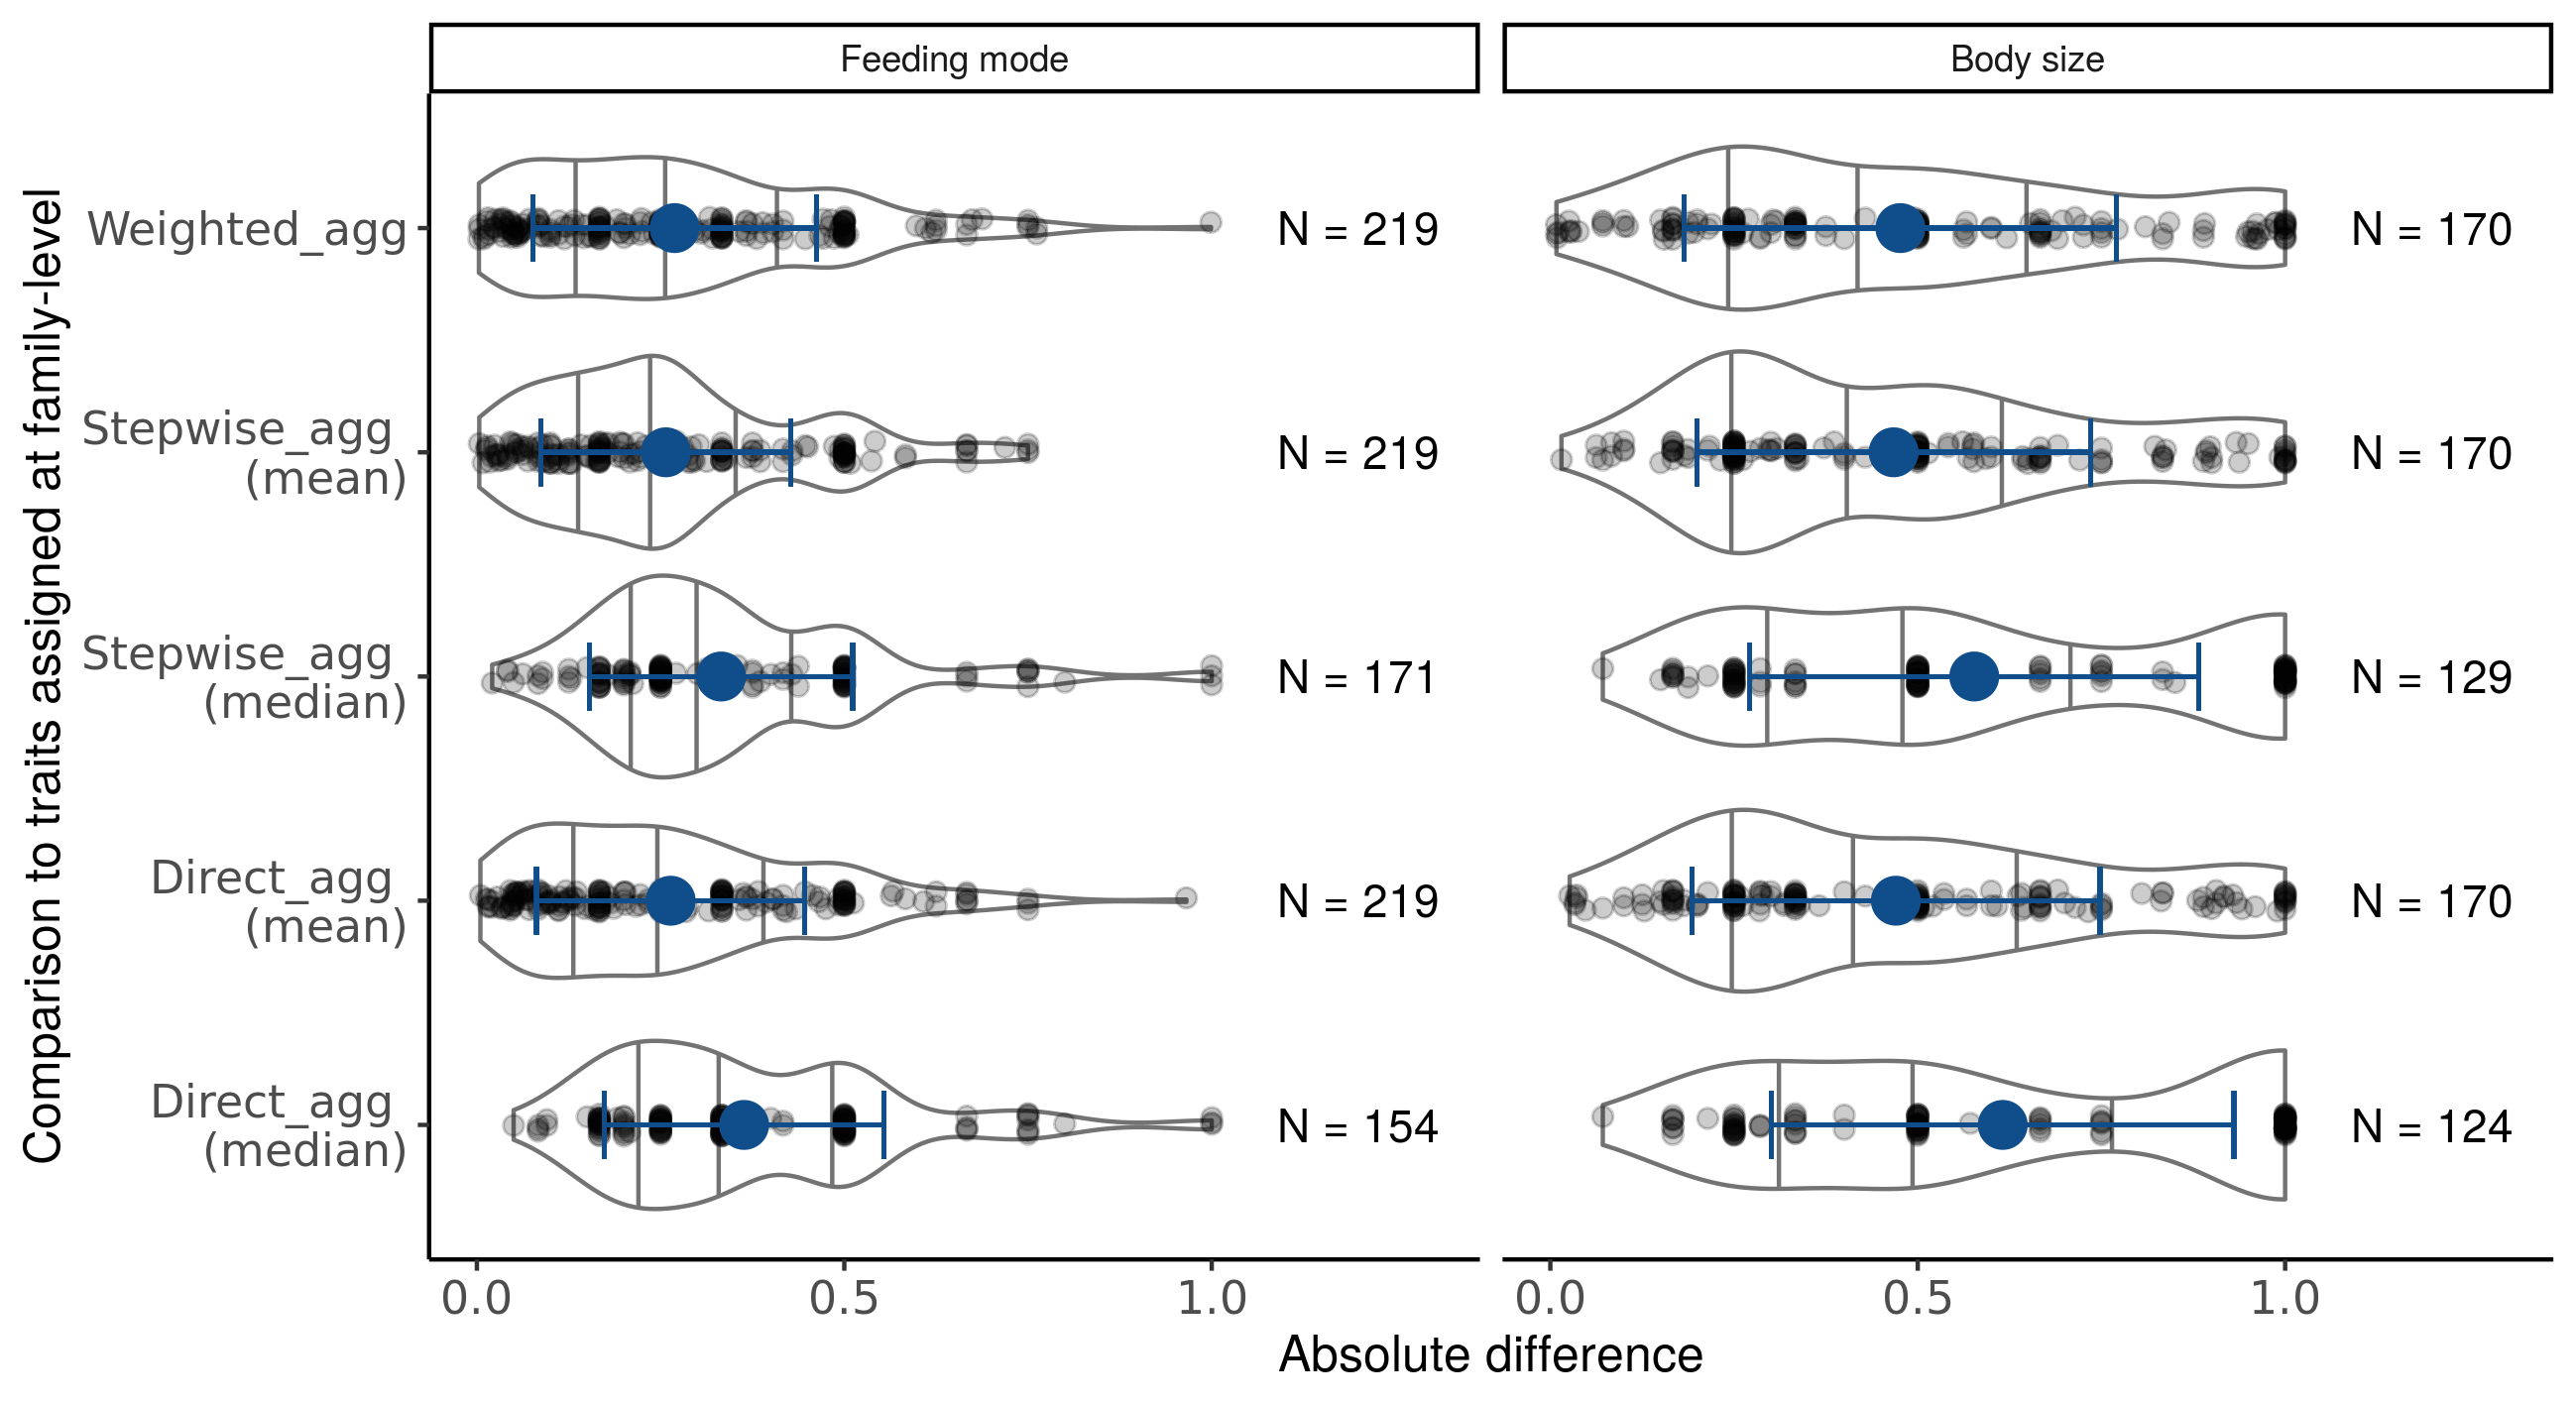
\includegraphics[width=16.5cm, height=10cm]{Deviances_trait_agg_chessman.png}
  \caption{Absolute differences in trait affinities between aggregated traits and traits assigned at family-level by Chessman et al. \cite{chessman_dissolved-oxygen_2018} for the grouping features feeding mode and body size. N denotes the number of cases for each comparison. The black dot indicates the mean absolute difference, the error bars the standard deviation. The gray horizontal lines show the 25th, 50th and 75th quantile of the density estimate.}
  \label{fig:diff_aggr_traits_chessman}
\end{figure}


\begin{figure}[H]
  \centering
  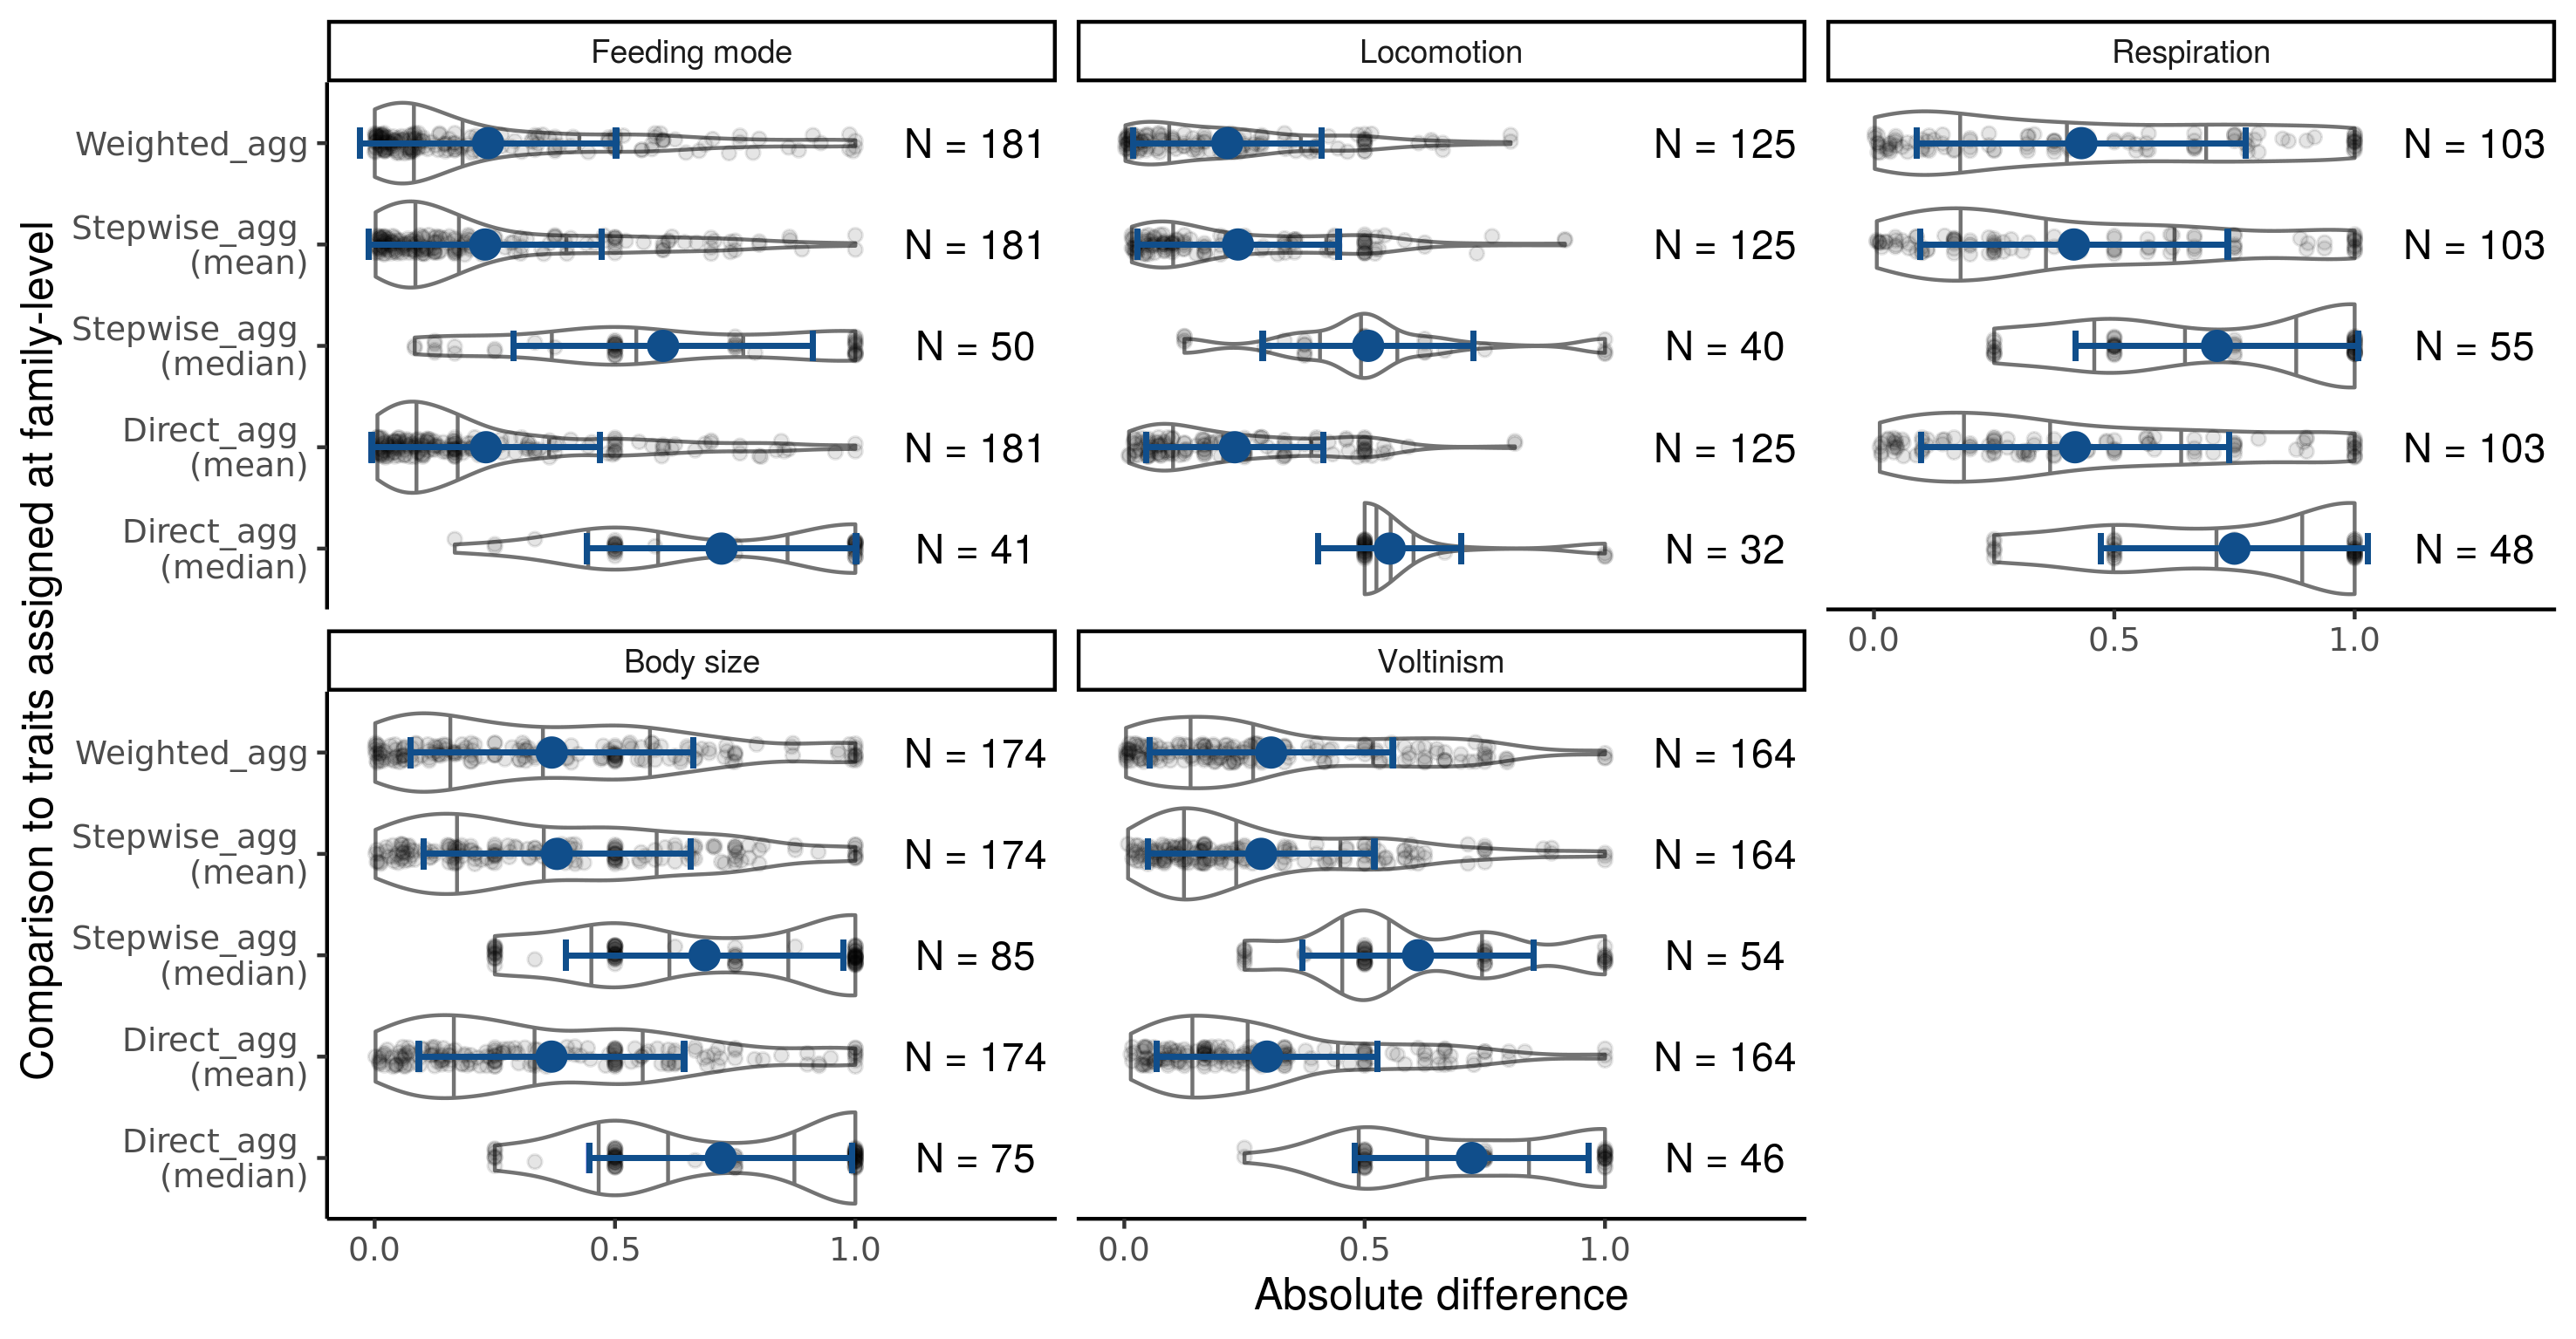
\includegraphics[width=16.5cm, height=10cm]{Deviances_trait_agg_pyne.png}
  \caption{Absolute differences in trait affinities between aggregated traits and traits assigned at family-level in the North American dataset for the grouping features feeding mode, locomotion, respiration, body size and voltinism. N denotes the number of cases for each comparison. The black dot indicates the mean absolute difference, the error bars the standard deviation. The gray horizontal lines show the 25th, 50th and 75th quantile of the density estimate.}
  \label{fig:diff_aggr_traits_pyne}
\end{figure}


\end{document}